%\documentclass[twoside]{thesisby}
\documentclass[oneside]{thesisby}

%верстка на A4 с указанными полями. После сжатия формата на А5 получатся поля по требованиям типографии БНТУ
\geometry{a4paper, left=2.5121cm, right=2.5121cm, bottom=2.645714cm, top=3.2114285cm}

\headsep = 14pt  %2,2628 %от текста до колонитутла

%\headheight = %высота колонтитула


%Шрифты тоже немного отмасштабируем
%\renewcommand{\tiny}{\fontsize{7}{8.4pt}\selectfont}
%\renewcommand{\scriptsize}{\fontsize{9}{11pt}\selectfont}
\renewcommand{\footnotesize}{\fontsize{12}{13.6pt}\selectfont}
\renewcommand{\small}{\fontsize{12}{13.6pt}\selectfont}
\renewcommand{\normalsize}{\fontsize{14.85}{17pt}\selectfont}
%\renewcommand{\large}{\fontsize{17}{20pt}\selectfont}
%\renewcommand{\Large}{\fontsize{20}{25pt}\selectfont}
%\renewcommand{\LARGE}{\fontsize{25}{30pt}\selectfont}

%%%и абзацный отступ тоже
\parindent=0.70946cm



%от рисунка до текста
\setlength{\textfloatsep}{0pt}


\fancypagestyle{plain}{%
%	\addtolength{\headheight}{\baselineskip}
\fancyhf{} % clear all header and footer fields
\fancyhead[C]{\hspace{10mm} \thepage} % except the center
\renewcommand{\headrulewidth}{0pt}
\renewcommand{\footrulewidth}{0pt}
}
\pagestyle{plain}

\setcounter{page}{-1} % начать нумерацию с номера три


%запрет висячих строк
%\clubpenalty=10000
%\widowpenalty=10000



\usepackage[utf8]{inputenc}
\usepackage[T1,T2A]{fontenc}
\usepackage[english, russian]{babel}

%для борьбы с переполнениями за счет разреженных слов в абзаце
\emergencystretch=25pt

\usepackage{amsmath,amssymb,amsfonts}

\usepackage{longtable,array}

\usepackage{graphicx,epsfig}

%раскоментить при создании электронной версии с гиперссылками
%%%%%%%%%%\usepackage[unicode,colorlinks,pagebackref]{hyperref}
%\usepackage[unicode]{hyperref}

%%%\usepackage{refcheck}% checks lost and useless labels, shows `keys' of \label in the margins

\usepackage{textcomp}% For Celsium sign only \textcelsius

\graphicspath{{fig/}}


\usepackage{multirow}

\usepackage{setspace}
% одинарный интервал
\singlespacing
% полуторный интервал
%\onehalfspacing
% двойной интервал
%\doublespacing
% произвольный интервал
%\setstretch{line_spacing_value}
%\setstretch{1.0}
%Для блока с текстом, например, можно сжать часть текста по вертикале
%\begin{singlespacing}
%...
%\end{singlespacing}
%или
%\begin{spacing}{1.0}
%...
%\end{spacing}

%последовательно переносы в строках
\doublehyphendemerits=10000

%-------


%Замечу, что пробел между словами "резиновое расстояние" (растягивается и сжимается). Пакет microtype помогает оптимизации. Просто загрузите -- и все
\usepackage{microtype}

%как сделать в латехе чтобы он писал [1-10]? 
%\usepackage{cite}  % \cite{Petrov, Sidorov...}


%%will be using font like `Times New Roman'
\usepackage{pscyr}
\renewcommand{\rmdefault}{ftm}

%%%current file is THESIS?
%%%YES - isthesis=1
%%%NO - isthesis=0
\usepackage{ifthen}
\newcounter{isthesis}
\setcounter{isthesis}{0}


%%%для времени сборки на титульном черновика
\usepackage{datetime}

\title{Изучение возможностей использования каши в голове в качестве пищи для ума}
\author{Вега Винсент Траволтович}
\date{\currenttime}
%%%\maketitle

%чтобы зачеркивать слова
\usepackage{ulem}
% в тексте, чтобы вычеркнуть слово
%\sout{Неправильно.} Правильно.

%%%%%поворот страницы альбомом
\usepackage{lscape}


     
      

\hyphenation{НИИСФ БНТУ МГСУ НИПТИС}


%%https://dxdy.ru/post985777.html#p985777

%% Определяем свой шрифт "greek"
\DeclareSymbolFont{greek}{U}{eur}{m}{n}
\SetSymbolFont{greek}{bold}{U}{eur}{b}{n}
\DeclareSymbolFontAlphabet{\gr}{greek}

%% Определяем буквы
\DeclareMathSymbol{\alpha}{\mathord}{greek}{"0B}
\DeclareMathSymbol{\beta}{\mathord}{greek}{"0C}
\DeclareMathSymbol{\gamma}{\mathord}{greek}{"0D}
\DeclareMathSymbol{\delta}{\mathord}{greek}{"0E}
\DeclareMathSymbol{\epsilon}{\mathord}{greek}{"0F}
\DeclareMathSymbol{\zeta}{\mathord}{greek}{"10}
\DeclareMathSymbol{\eta}{\mathord}{greek}{"11}
\DeclareMathSymbol{\theta}{\mathord}{greek}{"12}
\DeclareMathSymbol{\iota}{\mathord}{greek}{"13}
\DeclareMathSymbol{\kappa}{\mathord}{greek}{"14}
\DeclareMathSymbol{\lambda}{\mathord}{greek}{"15}
\DeclareMathSymbol{\mu}{\mathord}{greek}{"16}
\DeclareMathSymbol{\nu}{\mathord}{greek}{"17}
\DeclareMathSymbol{\xi}{\mathord}{greek}{"18}
\DeclareMathSymbol{\pi}{\mathord}{greek}{"19}
\DeclareMathSymbol{\rho}{\mathord}{greek}{"1A}
\DeclareMathSymbol{\sigma}{\mathord}{greek}{"1B}
\DeclareMathSymbol{\tau}{\mathord}{greek}{"1C}
\DeclareMathSymbol{\upsilon}{\mathord}{greek}{"1D}
\DeclareMathSymbol{\phi}{\mathord}{greek}{"1E}
\DeclareMathSymbol{\chi}{\mathord}{greek}{"1F}
\DeclareMathSymbol{\psi}{\mathord}{greek}{"20}
\DeclareMathSymbol{\omega}{\mathord}{greek}{"21}
\DeclareMathSymbol{\varepsilon}{\mathord}{greek}{"22}
\DeclareMathSymbol{\vartheta}{\mathord}{greek}{"23}
\DeclareMathSymbol{\varpi}{\mathord}{greek}{"24}
%% В AMS-овском шрифте  \varrho и \varsigma нет
\let\varrho\rho
\let\varsigma\sigma
\DeclareMathSymbol{\varphi}{\mathord}{greek}{"27}
%%https://dxdy.ru/post986322.html#p986322

%%%%%%%%%%%%%%%%%%%%%%%%%%%%%%%%%%%%%%%%%%%%%%%%%%%%%%%%%%%%%%%%%%%%%%%%%%
%%%                                                                    %%%
%%%              Вставить эти макрокоманды в преамбулу                 %%%
%%%                                                                    %%%
%%%%%%%%%%%%%%%%%%%%%%%%%%%%%%%%%%%%%%%%%%%%%%%%%%%%%%%%%%%%%%%%%%%%%%%%%%
%%%%%%%%%%%%%%%%%%%%%%%%%%%%%%%%%%%%%%%%%%%%%%%%%%%%%%%%%%%%%%%%%%%%%%%%%%
%                                                                      %%%
%%%  Задаем новый шрифт (для автоматического масштабирования индексов) %%%
%                                                                      %%%
\DeclareFontFamily{OT1}{mygreek}{}%                                    %%%
\DeclareFontShape{OT1}{mygreek}{m}{n}{<->omsegr}{}%                    %%%
\DeclareSymbolFont{Greekrm}{OT1}{mygreek}{m}{n}                        %%%
%                                                                      %%%
%%%  Переопределяем греческие буквы, в т.ч. большие (например, \Omega  %%%
%%%  в оригинале плохая, остальные переопределяем для единства стиля)  %%%
%                                                                      %%%
\DeclareMathSymbol{\Alpha}{\mathalpha}{Greekrm}{65}                    %%%
\DeclareMathSymbol{\Beta}{\mathalpha}{Greekrm}{66}                     %%%
\DeclareMathSymbol{\Gamma}{\mathalpha}{Greekrm}{71}                    %%%
\DeclareMathSymbol{\Delta}{\mathalpha}{Greekrm}{68}                    %%%
\DeclareMathSymbol{\Epsilon}{\mathalpha}{Greekrm}{69}                  %%%
\DeclareMathSymbol{\Zeta}{\mathalpha}{Greekrm}{90}                     %%%
\DeclareMathSymbol{\Eta}{\mathalpha}{Greekrm}{72}                      %%%
\DeclareMathSymbol{\Theta}{\mathalpha}{Greekrm}{74}                    %%%
\DeclareMathSymbol{\Iota}{\mathalpha}{Greekrm}{73}                     %%%
\DeclareMathSymbol{\Kappa}{\mathalpha}{Greekrm}{75}                    %%%
\DeclareMathSymbol{\Lambda}{\mathalpha}{Greekrm}{76}                   %%%
\DeclareMathSymbol{\Mu}{\mathalpha}{Greekrm}{77}                       %%%
\DeclareMathSymbol{\Nu}{\mathalpha}{Greekrm}{78}                       %%%
\DeclareMathSymbol{\Omicron}{\mathalpha}{Greekrm}{79}                  %%%
\DeclareMathSymbol{\Xi}{\mathalpha}{Greekrm}{88}                       %%%
\DeclareMathSymbol{\Pi}{\mathalpha}{Greekrm}{80}                       %%%
\DeclareMathSymbol{\Rho}{\mathalpha}{Greekrm}{82}                      %%%
\DeclareMathSymbol{\Sigma}{\mathalpha}{Greekrm}{83}                    %%%
\DeclareMathSymbol{\Tau}{\mathalpha}{Greekrm}{84}                      %%%
\DeclareMathSymbol{\Upsilon}{\mathalpha}{Greekrm}{85}                  %%%
\DeclareMathSymbol{\Phi}{\mathalpha}{Greekrm}{70}                      %%%
\DeclareMathSymbol{\Chi}{\mathalpha}{Greekrm}{81}                      %%%
\DeclareMathSymbol{\Psi}{\mathalpha}{Greekrm}{89}                      %%%
\DeclareMathSymbol{\Omega}{\mathalpha}{Greekrm}{87}                    %%%
%                                                                      %%%
\DeclareMathSymbol{\alpha}{\mathalpha}{Greekrm}{97}                    %%%
\DeclareMathSymbol{\beta}{\mathalpha}{Greekrm}{98}                     %%%
\DeclareMathSymbol{\varbeta}{\mathalpha}{Greekrm}{49}                  %%%
\DeclareMathSymbol{\gamma}{\mathalpha}{Greekrm}{103}                   %%%
\DeclareMathSymbol{\delta}{\mathalpha}{Greekrm}{100}                   %%%
\DeclareMathSymbol{\epsilon}{\mathalpha}{Greekrm}{101}                 %%%
\DeclareMathSymbol{\varepsilon}{\mathalpha}{Greekrm}{101}              %%%
\DeclareMathSymbol{\zeta}{\mathalpha}{Greekrm}{122}                    %%%
\DeclareMathSymbol{\eta}{\mathalpha}{Greekrm}{104}                     %%%
\DeclareMathSymbol{\theta}{\mathalpha}{Greekrm}{106}                   %%%
\DeclareMathSymbol{\vartheta}{\mathalpha}{Greekrm}{50}                 %%%
\DeclareMathSymbol{\iota}{\mathalpha}{Greekrm}{105}                    %%%
\DeclareMathSymbol{\kappa}{\mathalpha}{Greekrm}{107}                   %%%
\DeclareMathSymbol{\varkappa}{\mathalpha}{Greekrm}{53}                 %%%
\DeclareMathSymbol{\lambda}{\mathalpha}{Greekrm}{108}                  %%%
\DeclareMathSymbol{\mu}{\mathalpha}{Greekrm}{109}                      %%%
\DeclareMathSymbol{\nu}{\mathalpha}{Greekrm}{110}                      %%%
\DeclareMathSymbol{\omicron}{\mathalpha}{Greekrm}{111}                 %%%
\DeclareMathSymbol{\xi}{\mathalpha}{Greekrm}{120}                      %%%
\DeclareMathSymbol{\pi}{\mathalpha}{Greekrm}{112}                      %%%
\DeclareMathSymbol{\varpi}{\mathalpha}{Greekrm}{55}                    %%%
\DeclareMathSymbol{\rho}{\mathalpha}{Greekrm}{114}                     %%%
\DeclareMathSymbol{\varrho}{\mathalpha}{Greekrm}{52}                   %%%
\DeclareMathSymbol{\sigma}{\mathalpha}{Greekrm}{115}                   %%%
\DeclareMathSymbol{\varsigma}{\mathalpha}{Greekrm}{99}                 %%%
\DeclareMathSymbol{\tau}{\mathalpha}{Greekrm}{116}                     %%%
\DeclareMathSymbol{\upsilon}{\mathalpha}{Greekrm}{117}                 %%%
\DeclareMathSymbol{\phi}{\mathalpha}{Greekrm}{102}                     %%%
\DeclareMathSymbol{\varphi}{\mathalpha}{Greekrm}{51}                   %%%
\DeclareMathSymbol{\chi}{\mathalpha}{Greekrm}{113}                     %%%
\DeclareMathSymbol{\psi}{\mathalpha}{Greekrm}{121}                     %%%
\DeclareMathSymbol{\omega}{\mathalpha}{Greekrm}{119}                   %%%
%                                                                      %%%
%%%%%%%%%%%%%%%%%%%%%%%%%%%%%%%%%%%%%%%%%%%%%%%%%%%%%%%%%%%%%%%%%%%%%%%%%%
%%%%%%%%%%%%%%%%%%%%%%%%%%%%%%%%%%%%%%%%%%%%%%%%%%%%%%%%%%%%%%%%%%%%%%%%%%




\begin{document}
%ТИТУЛЬНЫЙ ЛИСТ
%\begin{titlepage}
\vspace{-26pt}
%\newpage
\pagestyle{empty}
\begin{center}
{БЕЛОРУССКИЙ\;НАЦИОНАЛЬНЫЙ\;ТЕХНИЧЕСКИЙ\;УНИВЕРСИТЕТ}
\end{center}
%\medskip

%\vspace{2cm}
~

~

%\noindent %На правах рукописи\\
\noindent УДК  000.00:000.000 \\

%\vspace{3cm}

~

~

~

~

~

~

~

\begin{center}
\noindent{\bfseries ВЕГА \\ Винсент Траволтович}\\

%\vspace{1cm}

~

~

\noindent{\bfseries ИЗУЧЕНИЕ ВОЗМОЖНОСТЕЙ\\ИСПОЛЬЗОВАНИЯ КАШИ В ГОЛОВЕ\\В КАЧЕСТВЕ ПИЩИ ДЛЯ УМА}\\ 
%\vspace{2.5cm}

~

~

~

~

~

~

\noindent{Автореферат \\ диссертации на соискание ученой степени\\
кандидата технических наук}\\

%ЧЕРНОВИК ПО СОСТОЯНИЮ НА \today ~ \currenttime \vspace{1cm}
%\vspace{2cm}


\noindent{
по специальности 00.00.00 -- Переворачивание пингвинов,\\дегустация алкоголя, и другие глупости в рабочее время
}
\end{center}



~

~

~

~

~

~

~

~

~


\begin{center}
 %\bfseries
\noindent Минск \the\year
\end{center}
%\end{titlepage}

%%\begin{titlepage}
\vspace{-26pt}
%\newpage
\pagestyle{empty}
\begin{center}
{БЕЛОРУССКИЙ\;НАЦИОНАЛЬНЫЙ\;ТЕХНИЧЕСКИЙ\;УНИВЕРСИТЕТ}
\end{center}
%\medskip

%\vspace{2cm}
~

~

%\noindent %На правах рукописи\\
\noindent УДК  000.00:000.000 \\

%\vspace{3cm}

~

~

~

~

~

~

~

\begin{center}
\noindent{\bfseries ВЕГА \\ Винсент Траволтович}\\

%\vspace{1cm}

~

~

\noindent{\bfseries ИЗУЧЕНИЕ ВОЗМОЖНОСТЕЙ\\ИСПОЛЬЗОВАНИЯ КАШИ В ГОЛОВЕ\\В КАЧЕСТВЕ ПИЩИ ДЛЯ УМА}\\ 
%\vspace{2.5cm}

~

~

~

~

~

~

\noindent{Автореферат \\ диссертации на соискание ученой степени\\
кандидата технических наук}\\

%ЧЕРНОВИК ПО СОСТОЯНИЮ НА \today ~ \currenttime \vspace{1cm}
%\vspace{2cm}


\noindent{
по специальности 00.00.00 -- Переворачивание пингвинов,\\дегустация алкоголя, и другие глупости в рабочее время
}
\end{center}



~

~

~

~

~

~

~

~

~


\begin{center}
 %\bfseries
\noindent Минск \the\year
\end{center}
%\end{titlepage}


%информация об оппонентах и др.
%\begin{titlepage}
\newpage
\pagestyle{empty}
Работа выполнена в Белорусском национальном техническом \linebreak университете

\vspace*{-4mm}
\begin{table*}[h!]
\hspace*{-4mm}
\begin{tabular}{p{65mm} p{94mm}}

{Научный руководитель} & {\textbf{ФАМИЛИЯ Имя Отчество}, доктор технических наук, профессор, профессор кафедры <<Ложки и молотки>> Белорусского национального технического университета} \tabularnewline 

~&~ \tabularnewline 

{Официальные оппоненты:} & \textbf{ФАМИЛИЯ Имя Отчество}, доктор технических наук, ведущий научный сотрудник, заместитель генерального директора Государственного предприятия <<Институт ПВТ \linebreak им.~Яндекса~С.~С.>>;
\tabularnewline 

~&~ \tabularnewline 

~ & \textbf{ФАМИЛИЯ Имя Отчество}, кандидат технических наук, доцент, заведующий кафедрой <<Вилки, ложки и решето>> УО~<<Гондурасский государственный технический университет >>
\tabularnewline 

~&~ \tabularnewline 

{Оппонирующая организация} & РУП~<<НАЗВАНИЕ>>

\end{tabular}
\end{table*}

\vspace*{-6mm}
Защита состоится
%<<\underline{~~~~~~}>> \underline{~~~~~~~~~~~~~~} 2019~г.
%в \underline{~~~~~~} часов
<<30>> февраля 2020~г.
в 10 часов
на заседании совета по защите диссертаций Д 00.00.00
при Белорусском государственном университете
по адресу: 220019, г.~Минск, пр-т~Франциска Скорины, 165, корп.~1, ауд.~1258,
тел. ученого секретаря \mbox{+375~17~000-00-00}.

С диссертацией можно ознакомиться в библиотеке Белорусского государственного университета.

Автореферат разослан <<\underline{~~~~~}>> \underline{~~~~~~~~~~~~~~} 2018~г.

\begin{table*}[h!]
\hspace*{-4mm}
\begin{tabular}{p{100mm} c r}
Ученый секретарь &
\multirow{3}*{{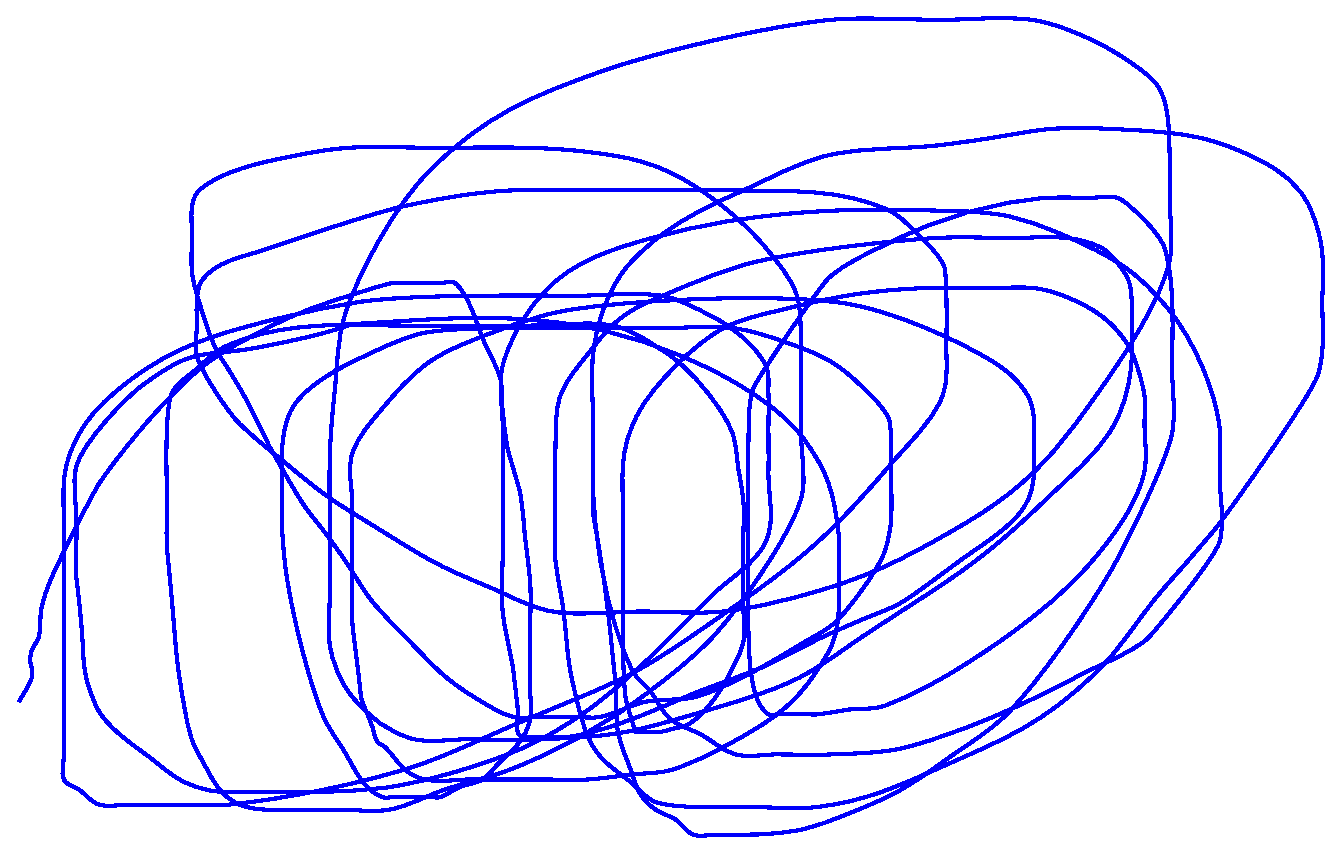
\includegraphics[width=3.5cm]{000sakratar_podpis}}}
&\\
совета по защите диссертаций, & &\\
доктор технических наук, профессор &  & И.~О.~Фамилия
\end{tabular}
\end{table*}
%
\vspace*{-3pt}
\begin{table*}[h!]
\hspace*{-4mm}
\begin{tabular}{p{80mm} l}
%
~ &  \copyright ~Вега~В.~Т., \the\year
\tabularnewline
~ & \copyright ~Белорусский национальный
\tabularnewline
~& ~~~~\,технический университет, \the\year
%
\end{tabular}
\end{table*}
%
%\end{titlepage}

\pagestyle{plain}

%ВВЕДЕНИЕ
%\begin{center}
\noindent\textbf{ВВЕДЕНИЕ}
\end{center}

~

Текст...
%~\\
\begin{center}
\noindent\textbf{ВВЕДЕНИЕ}
\end{center}

~

Текст...



%ОБЩАЯ ХАРАКТЕРИСТИКА РАБОТЫ
%остается как в диссере
%
%\newpage
\chapter*{ОБЩАЯ ХАРАКТЕРИСТИКА РАБОТЫ} ~
\addcontentsline{toc}{chapter}{ОБЩАЯ ХАРАКТЕРИСТИКА РАБОТЫ}~

\vspace{-16pt}
%\subsubsection*{Связь работы с научными программами (проектами), темами.}
\textbf{Связь работы с научными программами (проектами), темами}

Тема работы соответствует программе <<Переливание из пустого в порожнее>> приоритетных направлений научно-технической деятельности в Республике Беларусь на \mbox{2016--2020}~годы, утвержденных Указом Президента Республики Беларусь  \textnumero ~100500 от~30.02.2055.


\textbf{Цель и задачи исследования}

\textit{Цель работы}
-- откорректировать переработанный шаблон диссертации и залить в нет для его возможности использования другими поколениями ну и просто <<каб не прапала>>.

\textit{Объект исследований} -- абракадабра.

%\vspace{-20pt}
%\subsubsection*{Задачи исследований:}~
\textit{Задачи исследования:}

--~задачи исследования можно подгрузить из отдельного файла (прямо этого);

--~и его же можно подгрузить где-нибудь в литобзоре когда ставится задачи исследований;

--~хотя позже мне посоветовали текст задач изменить, чтобы не было дословного копирования из литобзора;

--~хотя, кому оно мешает в двух местах -- я так и не понял;

--~спишем на бюрократию.
%
%\ifthenelse{\value{isthesis}=0}{}{\pagebreak[4]}

%
%\vspace{-20pt}
%\subsubsection*{Научная новизна}работы:
%\pagebreak[4]
\textbf{Научная новизна} работы:

--~получены ...;

--~усовершенствована ...;

--~разработана ... .



%\vspace{-20pt}
%\subsubsection*{Положения, выносимые на защиту:}~
\ifthenelse{\value{isthesis}=0}{\pagebreak[4]}{}
\textbf{Положения, выносимые на защиту:}

--~результаты ...;

%\ifthenelse{\value{isthesis}=0}{\pagebreak[4]}{}

--~способ ...;

--~метод.


%\vspace{-20pt}
%\subsubsection*{Личный вклад соискателя.}~
\textbf{Личный вклад соискателя}~

Работа выполнена автором в Белорусском национальном техническом университете под руководством ...

Исследования ... проведены совместно с ...

Исследования ... выполнены совместно с ...

Остальные исследования ..., разработка математических моделей, ... и расчёты выполнены автором самостоятельно. 


%\vspace{-20pt}
%\subsubsection*{Апробация диссертации и информация об использовании ее результатов.}~
%\ifthenelse{\value{isthesis}=1}{\pagebreak[4]}{}
\textbf{Апробация диссертации и информация об использовании \linebreak ее результатов}~

Основные положения и результаты работы докладывались и обсуждались в рамках:

--~Научно-технических конференций <<ХХ>> \textnumero ~1--1 (2016--2019~гг.),  \textnumero ~1--5 (2002--2007~гг.);

--~V Международной практической конференции <<ХХ>>, Москва, 13 мая 2012~г.;

--~Научном семинаре <<ХХ>>, Санкт-Петербург, 23--24 июля 2001~г.;

--~Научно-практической конференции <<ХХ>>, Минск, 20 августа 2021~г.


%\vspace{-20pt}
%\subsubsection*{Опубликование результатов диссертации.}~
\textbf{Опубликование результатов диссертации}

По результатам работы опубликовано:

--\,пять статей в научных изданиях, соответствующих перечню ВАК Республики Беларусь;

--\,четыре статьи в научных изданиях, соответствующих перечню ВАК при Минобрнауки России;

--\,две статьи в научно-технических изданиях;

--\,пять публикаций в сборниках материалов и тезисов по результатам научно-технических конференций.


%\vspace{-20pt}
%\subsubsection*{Структура и объём диссертации.}~
\ifthenelse{\value{isthesis}=0}{\pagebreak[4]}{}
\textbf{Структура и объём диссертации}


Работа состоит из введения, общей характеристики работы, основной части, заключения,
списка использованных источников и приложений.

Основная часть работы состоит из 5 глав.

В первой главе выполнен ...

Вторая глава ...


В третьей главе ...


В главе 4 ...

\ifthenelse{\value{isthesis}=1}{\pagebreak[4]}{}
В главе 5...


Объём диссертации составляет ХХ страницы, в том числе основная часть YY страниц.
Основная часть содержит ZZ рисунков и TT таблиц.

%~\\
~\\
\vspace{-10pt}
\input{abstractcharacteristics_readonly}



%ОСНОВНАЯ ЧАСТЬ:
%%
\begin{center}
\textbf{ОСНОВНАЯ ЧАСТЬ}
\end{center}

~

В \textbf{первой главе} диссертации 



%\pagebreak[4]
Во \textbf{второй главе} диссертации 



В \textbf{третьей главе} диссертации ...

\noindent ... система уравнений принимает вид

\vspace{-10pt}
\begin{equation}\label{eq:tempUn3d}
c_{T_M}\rho_{_M} = \frac{\partial T}{\partial \tau }
;
\end{equation}
%\vspace{-8pt}
\begin{equation}\label{eq:thetaUn3d}
c_{m_M}\!(\!\theta,T\!)\!\rho_{_M}\! = \frac{\partial \theta }{\partial \tau },
\end{equation}


%в условиях ограниченного места автореферата простые строки получаются плотнее чем eqrem

\noindent где~$c_{T_M}$ -- удельная теплоёмкость, Дж/(кг$\cdot^\circ$C);

\hspace{1mm}$\rho_{_M}$ -- плотность материала, кг/м$^3$;

...




%\newpage
\textbf{Четвертая глава} диссертации посвящена 



В \textbf{пятой главе} диссертации представлены



\vspace{-10pt}
\begin{figure}[h!]
\begin{center}
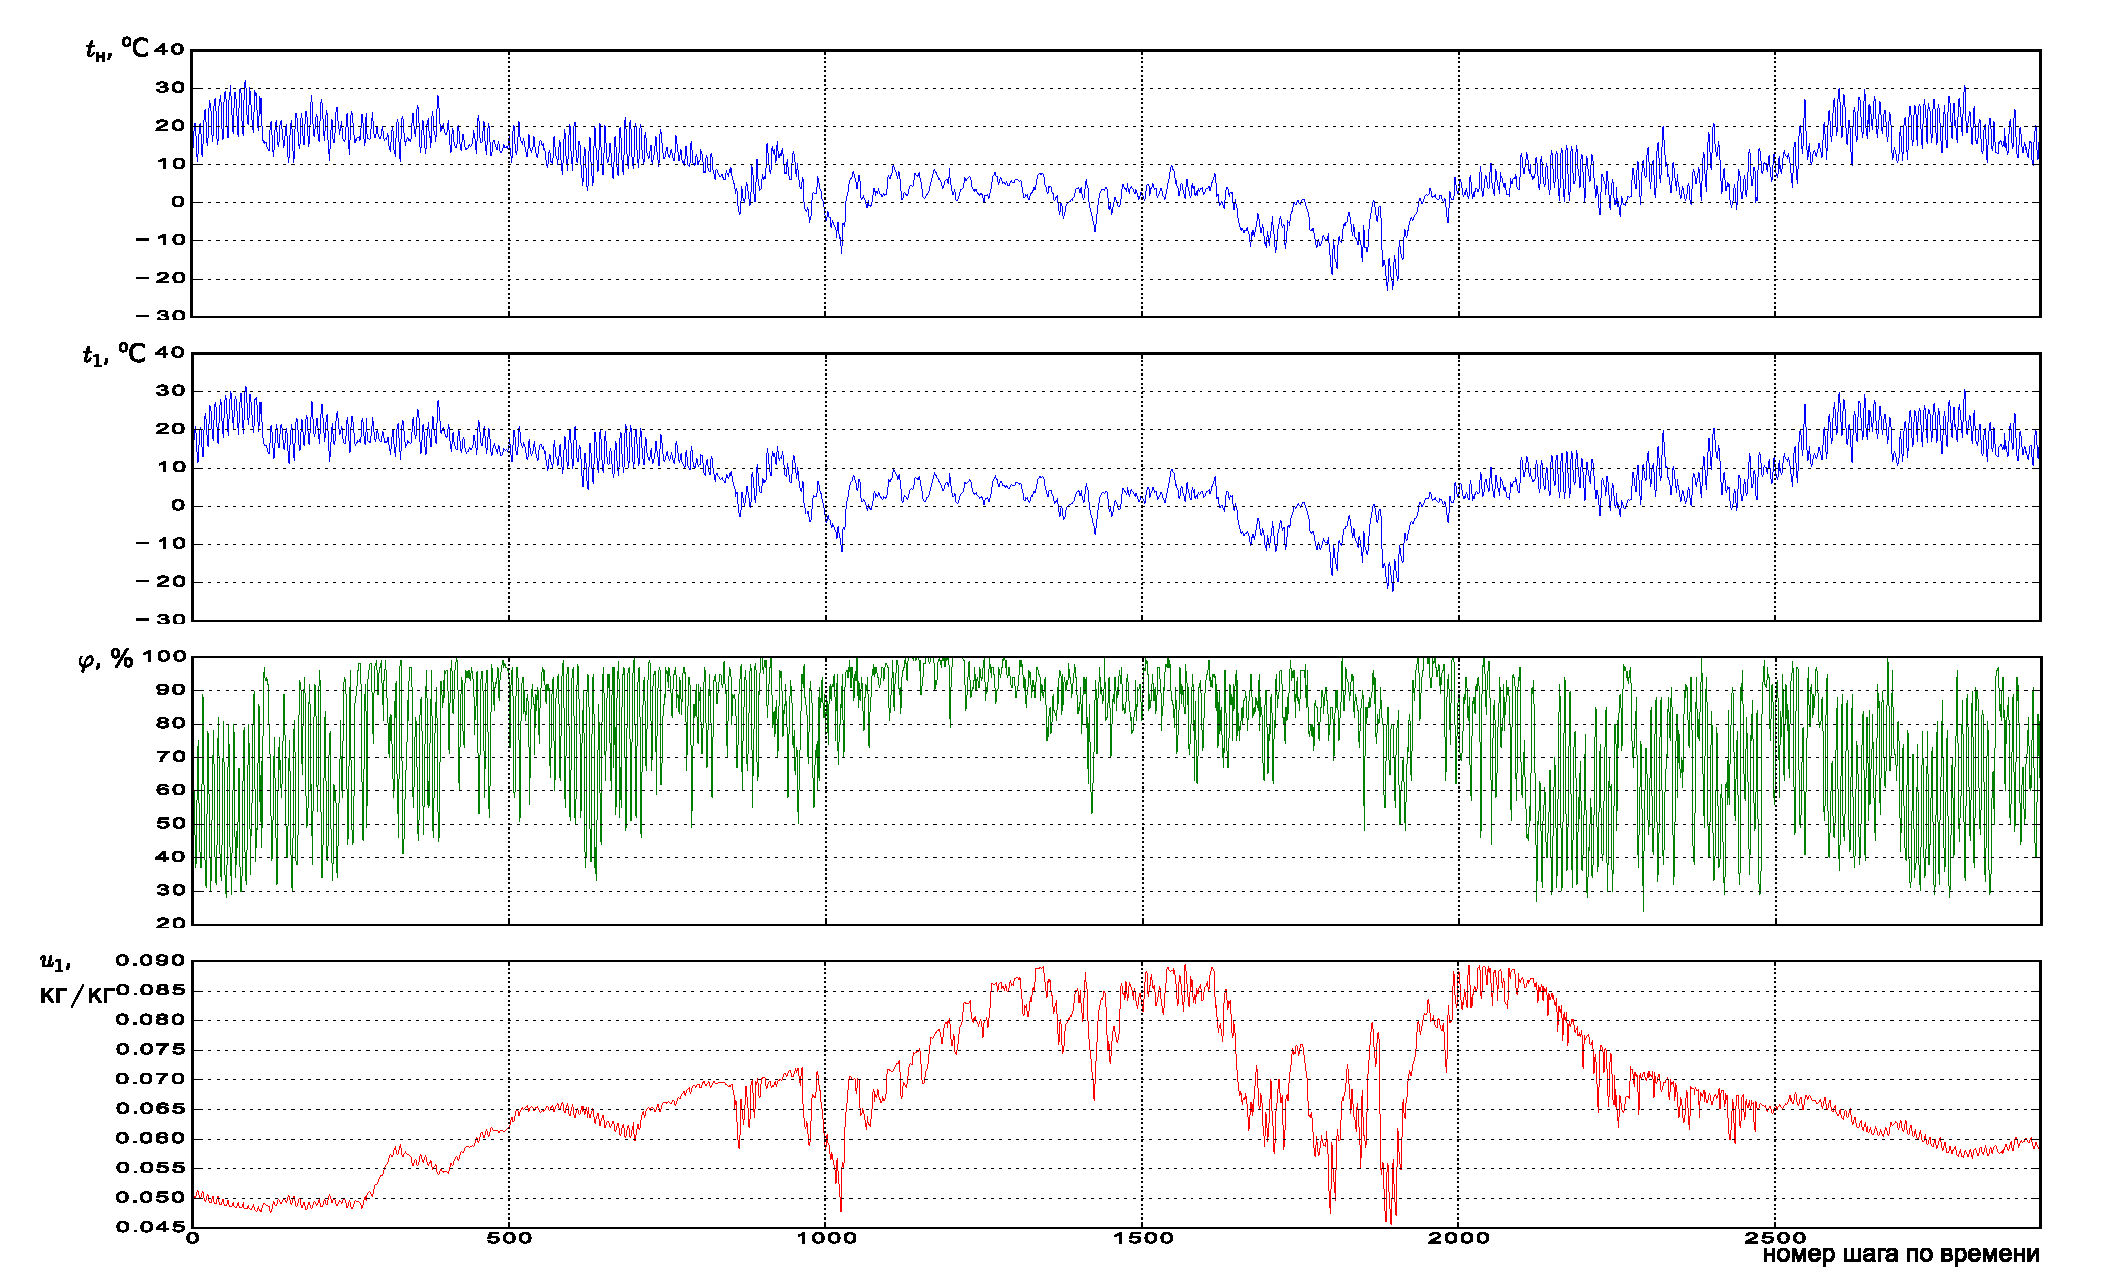
\includegraphics[angle=0,width=1.0\linewidth]{ch5-point1-1}\\[2mm]
\vspace{-10pt}
\caption {Рисунок сделан с помощью Matplotlib}\label{img:point1-1}
\end{center}
\end{figure}

...

~\\
\vspace{-10pt}
%
\begin{center}
\textbf{ОСНОВНАЯ ЧАСТЬ}
\end{center}

~

В \textbf{первой главе} диссертации 



%\pagebreak[4]
Во \textbf{второй главе} диссертации 



В \textbf{третьей главе} диссертации ...

\noindent ... система уравнений принимает вид

\vspace{-10pt}
\begin{equation}\label{eq:tempUn3d}
c_{T_M}\rho_{_M} = \frac{\partial T}{\partial \tau }
;
\end{equation}
%\vspace{-8pt}
\begin{equation}\label{eq:thetaUn3d}
c_{m_M}\!(\!\theta,T\!)\!\rho_{_M}\! = \frac{\partial \theta }{\partial \tau },
\end{equation}


%в условиях ограниченного места автореферата простые строки получаются плотнее чем eqrem

\noindent где~$c_{T_M}$ -- удельная теплоёмкость, Дж/(кг$\cdot^\circ$C);

\hspace{1mm}$\rho_{_M}$ -- плотность материала, кг/м$^3$;

...




%\newpage
\textbf{Четвертая глава} диссертации посвящена 



В \textbf{пятой главе} диссертации представлены



\vspace{-10pt}
\begin{figure}[h!]
\begin{center}
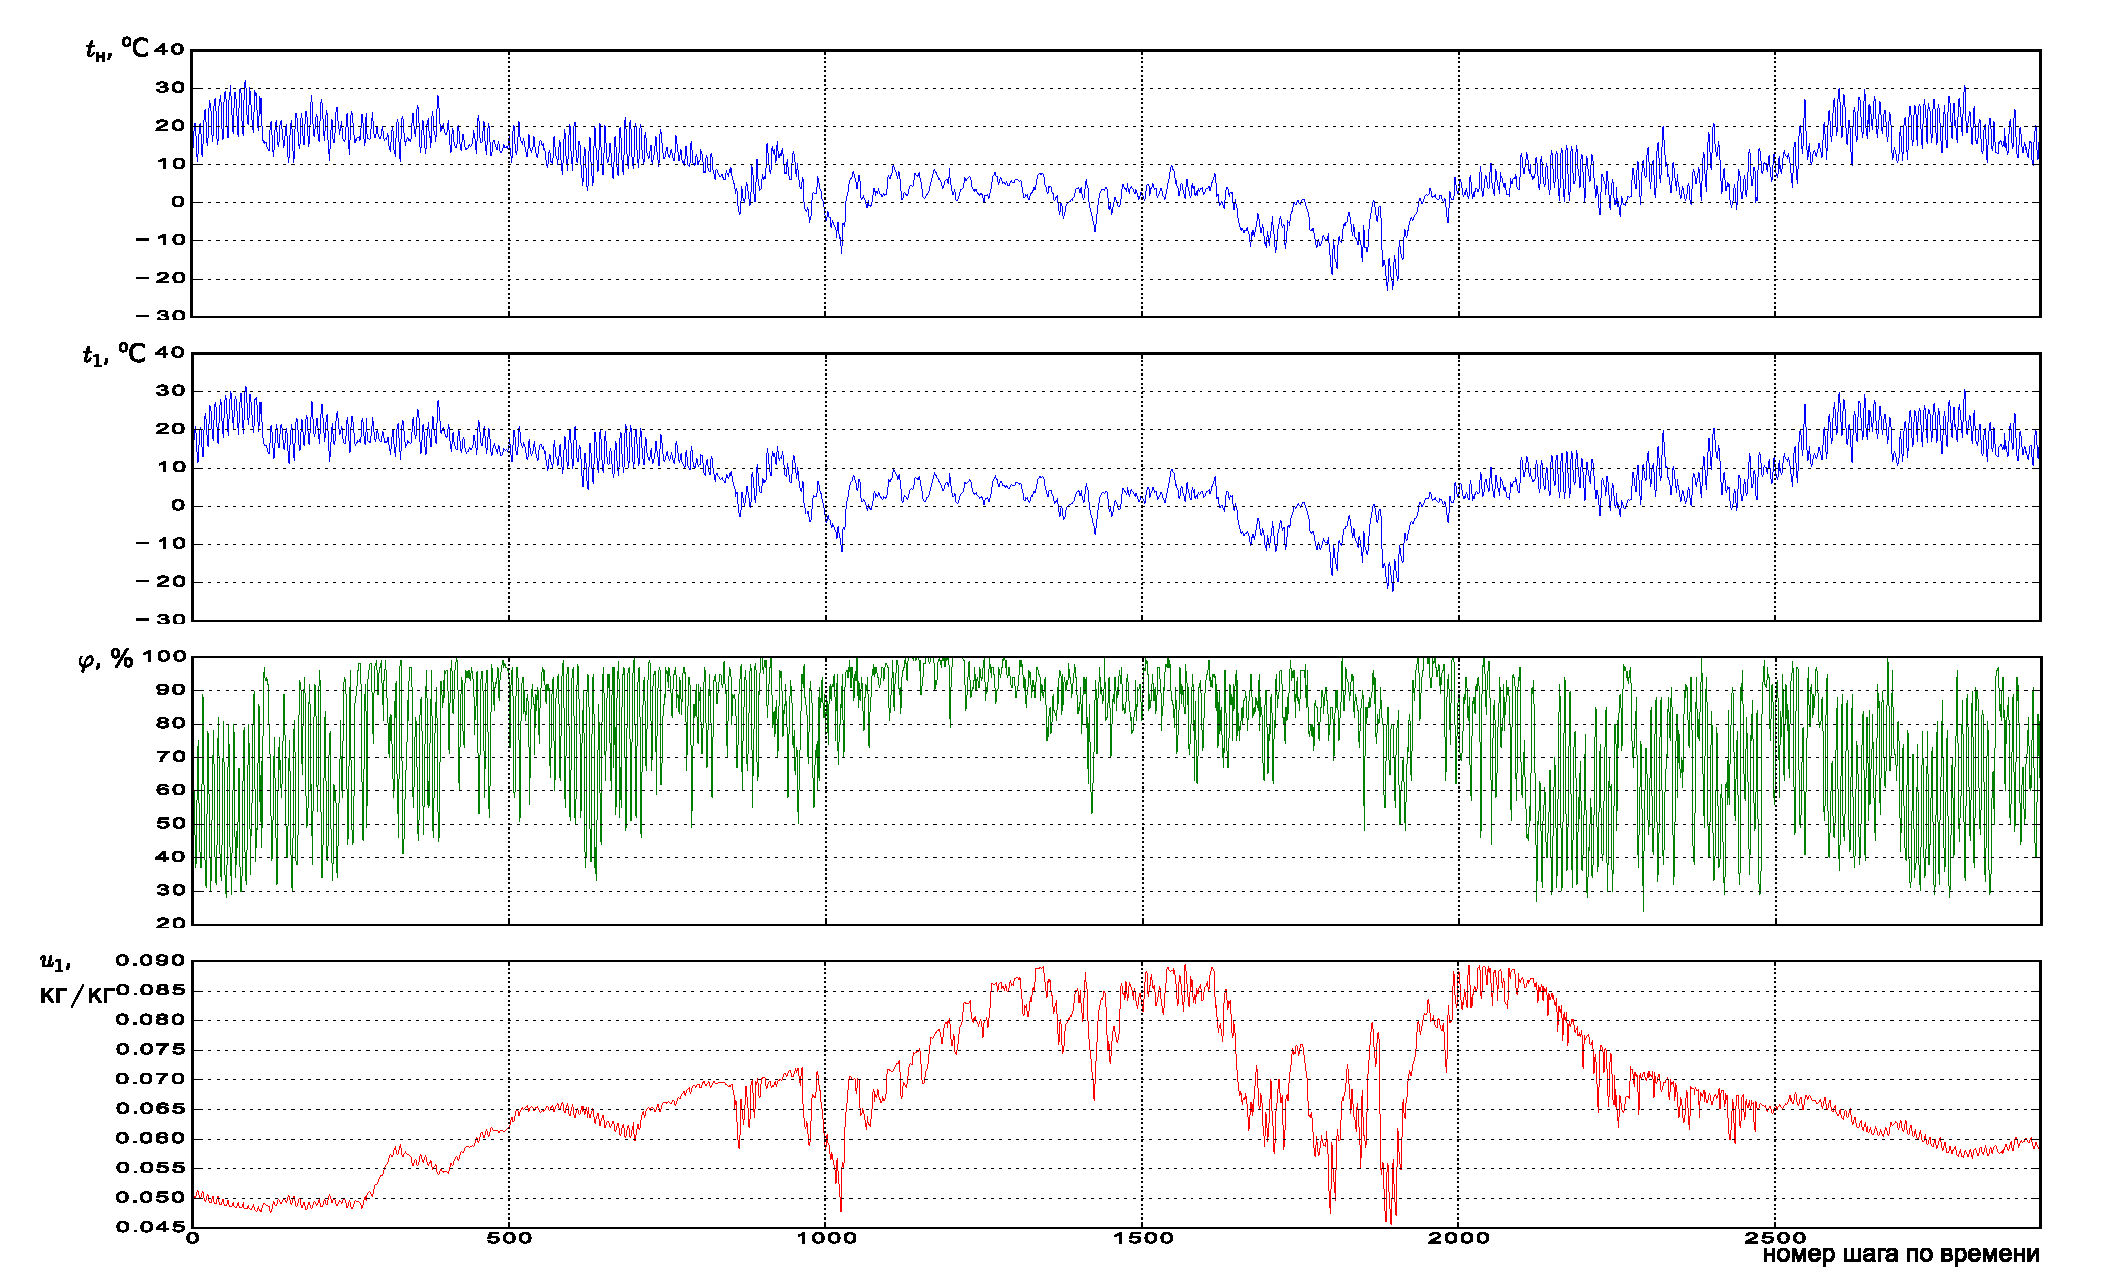
\includegraphics[angle=0,width=1.0\linewidth]{ch5-point1-1}\\[2mm]
\vspace{-10pt}
\caption {Рисунок сделан с помощью Matplotlib}\label{img:point1-1}
\end{center}
\end{figure}

...


%ЗАКЛЮЧЕНИЕ
%остаётся как в диссере
%\include{abstractconclusions_readonly}
~\\
\vspace{-20pt}
\input{abstractconclusions_readonly}
%~\\
%\newpage
%\chapter*{ЗАКЛЮЧЕНИЕ}
\addcontentsline{toc}{chapter}{ЗАКЛЮЧЕНИЕ}

\vspace{-10pt}
\subsection*{Основные научные результаты диссертации}

\vspace{-16pt}
%\subsubsection*{1.}
\textbf{1.~}
О-го-го!!!~\cite{myarticle1, myarticle2}.


\textbf{2.~}
Э-ге-гей!~\cite{myarticle3, myarticle4, myarticle5}.

Хе-хе-хе!!!~\cite{myarticle4, myarticle5}.


\textbf{3.~}
Э-э-эх!~\cite{myarticle6}.




\vspace{-10pt}
\ifthenelse{\value{isthesis}=1}{\newpage}{}
\subsection*{Рекомендации по практическому использованию результатов}

\vspace{-16pt}

У-у-ух!


%БИБЛИОГРАФИЧЕСКИЙ СПИСОК
% не нужен?????????????????!!!!!!!!!!!!!!!!
%\chapter*{БИБЛИОГРАФИЧЕСКИЙ СПИСОК}
%\addcontentsline{toc}{chapter}{БИБЛИОГРАФИЧЕСКИЙ СПИСОК}

%Библиография соискателя
%\bibliographystyle{gost71s2003}
%\bibliography{bibliographymy}
%\include{mybib}
%\newpage
%%\renewcommand{\mybibname}{}

\begin{center}{\textbf{СПИСОК ПУБЛИКАЦИЙ СОИСКАТЕЛЯ}}\end{center}
\addcontentsline{toc}{section}{Список публикаций соискателя}%

\renewcommand{\mybibname}{\normalsize \mbox{Статьи} в \mbox{изданиях,} \mbox{включенных} в \mbox{перечни} \mbox{научных} \mbox{изданий} \mbox{для опубликования} \mbox{результатов} \mbox{диссертационных} \mbox{исследований}}

\begin{myabstractbibliography}{10}
\def\selectlanguageifdefined#1{
\expandafter\ifx\csname date#1\endcsname\relax
\else\language\csname l@#1\endcsname\fi}
\ifx\undefined\url\def\url#1{{\small #1}}\else\fi
\ifx\undefined\BibUrl\def\BibUrl#1{\url{#1}}\else\fi
\ifx\undefined\BibAnnote\long\def\BibAnnote#1{}\else\fi
\ifx\undefined\BibEmph\def\BibEmph#1{\emph{#1}}\else\fi


% #1
\bibitem{myarticle1}
\selectlanguageifdefined{russian}
Название~статьи 1 / ~А.~А.~Автор1, ~А.~А.~Автор2, ~А.~А.~Автор3. ~А.~А.~Автор4~// ~Название~ ~Журнала. "---
\newblock 2006. "---
\newblock {\cyr\textnumero}~8. "---\newblock {\cyr\CYRS.}~5--9.


%#2
\bibitem{myarticle2}
\selectlanguageifdefined{russian}
Название~статьи 2 / ~А.~А.~Автор1, ~А.~А.~Автор2, ~А.~А.~Автор3, ~А.~А.~Автор4~// ~Название~ ~Журнала. "---
\newblock 2006. "---
\newblock {\cyr\textnumero}~8. "---\newblock {\cyr\CYRS.}~5--9.



\end{myabstractbibliography}


\renewcommand{\mybibname}{\normalsize \mbox{Статьи в научно-технических журналах}}

\begin{myabstractbibliography}{10}
\def\selectlanguageifdefined#1{
\expandafter\ifx\csname date#1\endcsname\relax
\else\language\csname l@#1\endcsname\fi}
\ifx\undefined\url\def\url#1{{\small #1}}\else\fi
\ifx\undefined\BibUrl\def\BibUrl#1{\url{#1}}\else\fi
\ifx\undefined\BibAnnote\long\def\BibAnnote#1{}\else\fi
\ifx\undefined\BibEmph\def\BibEmph#1{\emph{#1}}\else\fi

\setcounter{enumiv}{2} %тут вставить номер по порядку публикации из предыдущего раздела (здесь это номер 2  (см. выше %#2))

% #3
%эта НЕ ВАК
\bibitem{myarticle3}
\selectlanguageifdefined{russian}
Автор1,~А.~А. Влияние процессов ...~/ А.~А.~Автор1, А.~А.~Автор2~// 
  Журнал. "---
\newblock 2007. "---
\newblock {\cyr\textnumero} 7(40). "---
\newblock {\cyr\CYRS.}~58--61.

% #4
%эта НЕ ВАК
\bibitem{myarticle4}
\selectlanguageifdefined{russian}
Автор1,~А.~А. Влияние процессов ...~/ А.~А.~Автор1, А.~А.~Автор2, А.~А.~Автор3~// 
  Журнал. "---
\newblock 2013. "---
\newblock {\cyr\textnumero}~5. "---
\newblock {\cyr\CYRS.}~132--133.

\end{myabstractbibliography}



\renewcommand{\mybibname}{\normalsize \mbox{Материалы} \mbox{докладов} на \mbox{конференциях,} \mbox{семинарах,} \mbox{тезисы} \mbox{докладов}}

\begin{myabstractbibliography}{10}
\def\selectlanguageifdefined#1{
\expandafter\ifx\csname date#1\endcsname\relax
\else\language\csname l@#1\endcsname\fi}
\ifx\undefined\url\def\url#1{{\small #1}}\else\fi
\ifx\undefined\BibUrl\def\BibUrl#1{\url{#1}}\else\fi
\ifx\undefined\BibAnnote\long\def\BibAnnote#1{}\else\fi
\ifx\undefined\BibEmph\def\BibEmph#1{\emph{#1}}\else\fi

\setcounter{enumiv}{4} %тут вставить номер по порядку публикации из предыдущего раздела (здесь это номер 4)

%конференции

% #5
\bibitem{myarticle5}
\selectlanguageifdefined{russian}
Название ~/ А.~А.~Автор1, А.~А.~Автор2, А.~А.~Автор3,
  А.~А.~Автор4~// Наука -- образованию, производству, экономике: материалы
  Десятой междунар. науч.-техн. конф., Минск, 18–19 апр. 2006~г.: в~2~т.~/ Белорус. нац. техн. ун-т;
редкол.: И.~И.~Иванов, С.~С.~Сидоров, З.~З.~Забывайко. "---
\newblock \CYRT.~1. "---
\newblock Минск, 2006. "---
\newblock {\cyr\CYRS.}~11--19.

% #6
\bibitem{myarticle6}
\selectlanguageifdefined{russian}
Автор1,~А.~А. Название статьи~/ А.~А.~Автор1, А.~А.~Автор2~//
  Наука -- образованию, производству, экономике: материалы Пятой междунар. науч.-техн. конф., Минск, 11–12 апр. 2006~г.: в~12~т.~/ Белорус. нац. техн. ун-т;
редкол.: И.~И.~Иванов, С.~С.~Сидоров, З.~З.~Забывайко. "---
\newblock \CYRT.~1. "---
\newblock Минск, 2006. "---
\newblock {\cyr\CYRS.}~1--3.

\end{myabstractbibliography}

%\renewcommand{\mybibname}{}

\begin{center}{\textbf{СПИСОК ПУБЛИКАЦИЙ СОИСКАТЕЛЯ}}\end{center}
\addcontentsline{toc}{section}{Список публикаций соискателя}%

\renewcommand{\mybibname}{\normalsize \mbox{Статьи} в \mbox{изданиях,} \mbox{включенных} в \mbox{перечни} \mbox{научных} \mbox{изданий} \mbox{для опубликования} \mbox{результатов} \mbox{диссертационных} \mbox{исследований}}

\begin{myabstractbibliography}{10}
\def\selectlanguageifdefined#1{
\expandafter\ifx\csname date#1\endcsname\relax
\else\language\csname l@#1\endcsname\fi}
\ifx\undefined\url\def\url#1{{\small #1}}\else\fi
\ifx\undefined\BibUrl\def\BibUrl#1{\url{#1}}\else\fi
\ifx\undefined\BibAnnote\long\def\BibAnnote#1{}\else\fi
\ifx\undefined\BibEmph\def\BibEmph#1{\emph{#1}}\else\fi


% #1
\bibitem{myarticle1}
\selectlanguageifdefined{russian}
Название~статьи 1 / ~А.~А.~Автор1, ~А.~А.~Автор2, ~А.~А.~Автор3. ~А.~А.~Автор4~// ~Название~ ~Журнала. "---
\newblock 2006. "---
\newblock {\cyr\textnumero}~8. "---\newblock {\cyr\CYRS.}~5--9.


%#2
\bibitem{myarticle2}
\selectlanguageifdefined{russian}
Название~статьи 2 / ~А.~А.~Автор1, ~А.~А.~Автор2, ~А.~А.~Автор3, ~А.~А.~Автор4~// ~Название~ ~Журнала. "---
\newblock 2006. "---
\newblock {\cyr\textnumero}~8. "---\newblock {\cyr\CYRS.}~5--9.



\end{myabstractbibliography}


\renewcommand{\mybibname}{\normalsize \mbox{Статьи в научно-технических журналах}}

\begin{myabstractbibliography}{10}
\def\selectlanguageifdefined#1{
\expandafter\ifx\csname date#1\endcsname\relax
\else\language\csname l@#1\endcsname\fi}
\ifx\undefined\url\def\url#1{{\small #1}}\else\fi
\ifx\undefined\BibUrl\def\BibUrl#1{\url{#1}}\else\fi
\ifx\undefined\BibAnnote\long\def\BibAnnote#1{}\else\fi
\ifx\undefined\BibEmph\def\BibEmph#1{\emph{#1}}\else\fi

\setcounter{enumiv}{2} %тут вставить номер по порядку публикации из предыдущего раздела (здесь это номер 2  (см. выше %#2))

% #3
%эта НЕ ВАК
\bibitem{myarticle3}
\selectlanguageifdefined{russian}
Автор1,~А.~А. Влияние процессов ...~/ А.~А.~Автор1, А.~А.~Автор2~// 
  Журнал. "---
\newblock 2007. "---
\newblock {\cyr\textnumero} 7(40). "---
\newblock {\cyr\CYRS.}~58--61.

% #4
%эта НЕ ВАК
\bibitem{myarticle4}
\selectlanguageifdefined{russian}
Автор1,~А.~А. Влияние процессов ...~/ А.~А.~Автор1, А.~А.~Автор2, А.~А.~Автор3~// 
  Журнал. "---
\newblock 2013. "---
\newblock {\cyr\textnumero}~5. "---
\newblock {\cyr\CYRS.}~132--133.

\end{myabstractbibliography}



\renewcommand{\mybibname}{\normalsize \mbox{Материалы} \mbox{докладов} на \mbox{конференциях,} \mbox{семинарах,} \mbox{тезисы} \mbox{докладов}}

\begin{myabstractbibliography}{10}
\def\selectlanguageifdefined#1{
\expandafter\ifx\csname date#1\endcsname\relax
\else\language\csname l@#1\endcsname\fi}
\ifx\undefined\url\def\url#1{{\small #1}}\else\fi
\ifx\undefined\BibUrl\def\BibUrl#1{\url{#1}}\else\fi
\ifx\undefined\BibAnnote\long\def\BibAnnote#1{}\else\fi
\ifx\undefined\BibEmph\def\BibEmph#1{\emph{#1}}\else\fi

\setcounter{enumiv}{4} %тут вставить номер по порядку публикации из предыдущего раздела (здесь это номер 4)

%конференции

% #5
\bibitem{myarticle5}
\selectlanguageifdefined{russian}
Название ~/ А.~А.~Автор1, А.~А.~Автор2, А.~А.~Автор3,
  А.~А.~Автор4~// Наука -- образованию, производству, экономике: материалы
  Десятой междунар. науч.-техн. конф., Минск, 18–19 апр. 2006~г.: в~2~т.~/ Белорус. нац. техн. ун-т;
редкол.: И.~И.~Иванов, С.~С.~Сидоров, З.~З.~Забывайко. "---
\newblock \CYRT.~1. "---
\newblock Минск, 2006. "---
\newblock {\cyr\CYRS.}~11--19.

% #6
\bibitem{myarticle6}
\selectlanguageifdefined{russian}
Автор1,~А.~А. Название статьи~/ А.~А.~Автор1, А.~А.~Автор2~//
  Наука -- образованию, производству, экономике: материалы Пятой междунар. науч.-техн. конф., Минск, 11–12 апр. 2006~г.: в~12~т.~/ Белорус. нац. техн. ун-т;
редкол.: И.~И.~Иванов, С.~С.~Сидоров, З.~З.~Забывайко. "---
\newblock \CYRT.~1. "---
\newblock Минск, 2006. "---
\newblock {\cyr\CYRS.}~1--3.

\end{myabstractbibliography}

%
%
%~\\
%\newpage
%~\\
%\chapter*{\normalsize РЭЗЮМЭ}
\begin{center}
\textbf{РЭЗЮМЭ}
\end{center}

~

\vspace{-10pt}
\begin{center}
\textbf{Вега Вінцэнт Траволтавіч}
\end{center}

~

\vspace{-10pt}
\begin{center}
\textbf{Выкарыстанне магчымасці выкарыстання кашы ў галаве ў якасці сілкавання розуму}
\end{center}

~

\vspace{-10pt}
\textbf{Ключавыя словы:}
словы. словы, словы.


\textbf{Мэта работы:}
мэта.

\textbf{Метады даследвання:}
метады.

\textbf{Атрыманыя вынікі і іх навізна.}
Вынікі.

\textbf{Рэкамендацыі па выкарыстанні.}
Рэкамендацыі.

\textbf{Галіна выкарыстання:}
галіна.



\newpage
%\chapter*{\normalsize РЕЗЮМЕ}
\begin{center}
\textbf{РЕЗЮМЕ}
\end{center}

~

\vspace{-10pt}
\begin{center}
\textbf{Вега Винсент Траволтович}
\end{center}

~

\vspace{-10pt}
\begin{center}
\textbf{Изучение возможностей использования каши в голове в качестве пищи для ума}
\end{center}

~

\vspace{-10pt}
\textbf{Ключевые слова:}
слова, слова.


\textbf{Цель работы:}
цель.

\textbf{Методы исследования:}
методы.

\textbf{Полученные результаты и их новизна.}
Результаты.

\textbf {Рекомендации по использованию.}
Рекомендации.

\textbf{Область применения:}
область.


\newpage
\pagestyle{empty}
%\chapter*{\normalsize SUMMARY}
\begin{center}
\textbf{SUMMARY}
\end{center}

~

\vspace{-10pt}
\begin{center}
\textbf{Vega Vincent}
\end{center}

~

\vspace{-10pt}
\begin{center}
\textbf{Research of the possibilities of using porridge in the head as the food for the mind}
\end{center}

~

\vspace{-10pt}
\textbf{Keywords:}
words, words.


\textbf{Objective:}
objectives.

\textbf{Research Methods:}
methods.

\textbf{Obtained results and their novelty.}
Results.

\textbf {Recommendations for use.}
Recomendations.

\textbf{Application field:}
field.

\newpage
%~\\
%\chapter*{\normalsize РЭЗЮМЭ}
\begin{center}
\textbf{РЭЗЮМЭ}
\end{center}

~

\vspace{-10pt}
\begin{center}
\textbf{Вега Вінцэнт Траволтавіч}
\end{center}

~

\vspace{-10pt}
\begin{center}
\textbf{Выкарыстанне магчымасці выкарыстання кашы ў галаве ў якасці сілкавання розуму}
\end{center}

~

\vspace{-10pt}
\textbf{Ключавыя словы:}
словы. словы, словы.


\textbf{Мэта работы:}
мэта.

\textbf{Метады даследвання:}
метады.

\textbf{Атрыманыя вынікі і іх навізна.}
Вынікі.

\textbf{Рэкамендацыі па выкарыстанні.}
Рэкамендацыі.

\textbf{Галіна выкарыстання:}
галіна.



\newpage
%\chapter*{\normalsize РЕЗЮМЕ}
\begin{center}
\textbf{РЕЗЮМЕ}
\end{center}

~

\vspace{-10pt}
\begin{center}
\textbf{Вега Винсент Траволтович}
\end{center}

~

\vspace{-10pt}
\begin{center}
\textbf{Изучение возможностей использования каши в голове в качестве пищи для ума}
\end{center}

~

\vspace{-10pt}
\textbf{Ключевые слова:}
слова, слова.


\textbf{Цель работы:}
цель.

\textbf{Методы исследования:}
методы.

\textbf{Полученные результаты и их новизна.}
Результаты.

\textbf {Рекомендации по использованию.}
Рекомендации.

\textbf{Область применения:}
область.


\newpage
\pagestyle{empty}
%\chapter*{\normalsize SUMMARY}
\begin{center}
\textbf{SUMMARY}
\end{center}

~

\vspace{-10pt}
\begin{center}
\textbf{Vega Vincent}
\end{center}

~

\vspace{-10pt}
\begin{center}
\textbf{Research of the possibilities of using porridge in the head as the food for the mind}
\end{center}

~

\vspace{-10pt}
\textbf{Keywords:}
words, words.


\textbf{Objective:}
objectives.

\textbf{Research Methods:}
methods.

\textbf{Obtained results and their novelty.}
Results.

\textbf {Recommendations for use.}
Recomendations.

\textbf{Application field:}
field.


%\chapter*{ТИПОГРАФИЯ}

\newpage

\begin{titlepage}
~
\begin{center}

\vspace{60mm}
Научное издание

~

~

\textbf{ВЕГА}

\textbf{Винсент Траволтович}

~

\textbf{ИЗУЧЕНИЕ ВОЗМОЖНОСТЕЙ\\ИСПОЛЬЗОВАНИЯ КАШИ В ГОЛОВЕ\\В КАЧЕСТВЕ ПИЩИ ДЛЯ УМА}

~

Автореферат диссертации

на соискание ученой степени кандидата технических наук

по специальности 00.00.00 – Переворачивание пингвинов, дегустация алкоголя, и другие глупости в рабочее время


\vspace{30mm}

%\footnotesize {
%Подписано в печать XX.XX.201X.
%\\
%Формат 60х84 1/16. Бумага офсетная. Ризография.
%\\
%Усл. печ. л. 1,XX. Уч.-изд. л. 1,XX. Тираж X0. Заказ 8XX.
%}
%\\
%\hrulefill


%\footnotesize{
%Издатель и полиграфическое исполнение: Белорусский национальный технический университет.
%\\
%Свидетельство о государственной регистрации издателя, изготовителя, распространителя
%\\
%печатных изданий \textnumero 1/173 от 12.02.2014. Пр. Независимости, 65. 220013, г. Минск.
%}

\end{center}
\end{titlepage}


%ПРИЛОЖЕНИЯ
%\appendix
%\chapter{ОЦЕНИВАНИЕ НЕОПРЕДЕЛЕННОСТИ ИЗМЕРЕНИЙ...} \label{app_neopr}

%отмена выноса section в содержание
\settocdepth{chapter}


Согласно \cite{iso200898} процесс оценивания неопределенности можно представить в виде следующих этапов:

...

Результаты расчета представлены в виде таблицы \ref{table_uw}.




\begin{landscape}

\begin{table}[h]
\caption {Результаты расчёта неопределенности ...}
\label{table_uw}
\begin{center}
\begin{small}
\begin{spacing}{3}
\begin{tabular}{|c|c|c|c|c|c|c|c|c|c|c|c|c|}
\hline
{\textnumero ~слоя}
& {$u(m_\text{в+б})$, г}
& {$u(m_\text{c+б})$, г}
& {$u(m_\text{б})$, г}
& {$c_{m_\text{в+б}}$}
& {$c_{m_\text{с+б}}$}
& {$c_{m_\text{б}}$}
& {$u(w_s)$, \%}
& {$u(\delta w_v)$, \%}
& {$\overline{w}$, \%}
& {$u(w)$, \%}
& {$U(w)$, \%}
& {$w$, \%} \\
\hline


1&0,0115&0,0769&0,0115&0,918&-0,936&0,018&0,073&0,426&1,38&0,43&0,86& 1,38$\pm$0,86\\
\hline

2&0,0115&0,0775&0,0115&0,910&-0,957&0,047&0,075&0,127&3,67&0,15&0,29& 3,67$\pm$0,29\\
\hline

3&0,0115&0,0784&0,0115&0,901&-0,955&0,054&0,076&0,139&4,19&0,16&0,32& 4,19$\pm$0,32\\
\hline

4&0,0115&0,0797&0,0115&0,882&-0,929&0,047&0,075&0,130&3,78&0,15&0,30& 3,78$\pm$0,30\\
\hline

5&0,0115&0,0755&0,0115&0,940&-0,985&0,045&0,075&0,193&3,34&0,21&0,41& 3,34$\pm$0,41\\
\hline


\end{tabular}
\end{spacing}
\end{small}
\end{center}
\end{table}

\end{landscape}




\resettocdepth
\chapter{ЧТО-ТО ЕЩЁ}
\label{AppB}


В таблице \ref{tab_sorbc_gs} представлены значения ...




\begin{longtable}{|c|c|c|c|c|c|c|c|c|c|p{1.3cm}|}
\caption{Значения чего-то там при различной температуре}
\label{tab_sorbc_gs}
\\
\hline
Температура, & \multicolumn{10}{c|} {Некая величина, \%,}
\\
\textcelsius & \multicolumn{10}{c|} {при относительной влажности воздуха, \%}
\\
%\hline
{} & 10 &  33 &  40 &  55 &  75 &  80 &  85 &  90 &  97 & над водой\\
\hline
0 & - & - & - & - & 6,21 & - & - & - & - & -\\
\hline
2 & - & - & - & - & - & - & - & - & - & 178\\
\hline
1 & 0,20 & 1,00 & - & 10 & 15 & - & 20 & 50 & 100 & -\\
\hline
60 & - & - & - & - & 20 & - & - & - & - & -\\
\hline
-6 & - & - & 1,56 & - & - & 25 & - & - & - & -\\
\hline
-0 & - & - & - & - & - & 9,0 & - & - & 8,3 & -\\
\hline
\end{longtable}





\chapter{ИНФОРМАЦИЯ О ПРАКТИЧЕСКОМ ИСПОЛЬЗОВАНИИ РЕЗУЛЬТАТОВ РАБОТЫ} \label{app_vnedr}

Цветные сканы актов и справок о внедрениях с крупной надписью\\ <<КОПИЯ>>.





\end{document}


